
%
% Proton_Attractive_Force
%
\begin{figure}
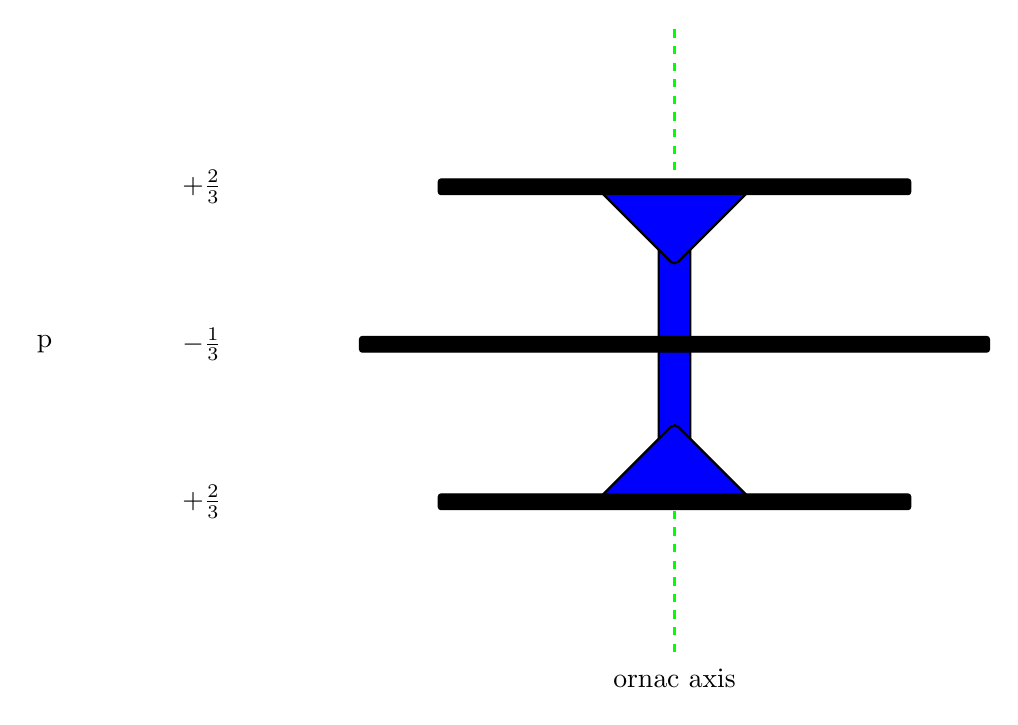
\begin{tikzpicture}[scale=1, rotate=0]


% Ornac axis
\draw[green, dashed, very thick] (4,6) -- (4,-2) ;
\path 
(4,-2) node [below]  {ornac axis};




\path 
(-4,2) node   {p};




% Up quark ornac-pair
\path 
(-2,4) node  (red) {$+\frac{2}{3}$};

% Blue rect to show force
\filldraw[fill=blue, draw=black, thick,rounded corners=2pt] (3.8, 4) rectangle (4.2, 0);

% Blue arrow down
\filldraw[fill=blue, draw=black, thick,rounded corners=2pt] (3,4) -- (5,4) -- (4,3)-- cycle; 

\filldraw[fill=black, draw=black ,rounded corners=1pt] (1, 3.9) rectangle (7, 4.1);


% Down quark ornac-pair
\path 
(-2,2) node  (red) {$-\frac{1}{3}$};

% Red arrow up
%\filldraw[fill=red, draw=black, thick,rounded corners=2pt] (3,2) -- (5,2) -- (4,3)-- cycle; 

% Red arrow down
%\filldraw[fill=red, draw=black, thick,rounded corners=2pt] (3,2) -- (5,2) -- (4,1)-- cycle; 

\filldraw[fill=black, draw=black ,rounded corners=1pt] (0, 1.9) rectangle (8, 2.1);


% Up quark ornac-pair
\path 
(-2,0) node  (red) {$+\frac{2}{3}$};

% Blue arrow up
\filldraw[fill=blue, draw=black, thick,rounded corners=2pt] (3,0) -- (5,0) -- (4,1)-- cycle; 
   

\filldraw[fill=black, draw=black ,rounded corners=1pt] (1,-0.1) rectangle (7, 0.1);





\end{tikzpicture}
\caption{Proton Attractive Force. When charges of the same polarity circle along the same axis and
 in the same direction of rotation, they create magnetic fields, which pull them together.
\label{Fig:Proton_Attractive_Force}}
\end{figure}



